\documentclass[conference]{IEEEtran}
\IEEEoverridecommandlockouts
\usepackage{cite}
\usepackage{amsmath,amssymb,amsfonts}
\usepackage{algorithmic}
\usepackage{graphicx}
\usepackage{textcomp}
\usepackage{xcolor}
\usepackage{hyperref}
\def\BibTeX{{\rm B\kern-.05em{\sc i\kern-.025em b}\kern-.08em
    T\kern-.1667em\lower.7ex\hbox{E}\kern-.125emX}}
\begin{document}

\title{Design, Implementation, and Analysis of an AM Modulator and Demodulator\\
{\Large Electronic Workshop 2 - Project 2}
}


\author{\IEEEauthorblockN{\textbf{Chamarthy Madhan Sai Krishna}}
\IEEEauthorblockA{\textit{Electronics \& Communication Engineering} \\
\textit{IIIT Hyderabad}\\
chamarthymadhan.k@students.iiit.ac.in\\2023102030}
\and
\IEEEauthorblockN{\textbf{Sajiv Singh}}
\IEEEauthorblockA{\textit{Electronics \& Communication Engineering} \\
\textit{IIIT Hyderabad}\\
sajiv.singh@research.iiit.ac.in\\2023112003}
}
\maketitle

\begin{abstract}

The project focuses on the design, implementation and analysis of a Double Sideband Suppressed Carrier (DSB-SC) Amplitude Modulation(AM) modulator and demodulator circuit prototype.

The main goal was to modulate the carrier signal, generated by the Local Oscillator (LO), using the modulating signal from the DSO, and to successfully recover the original signal.

Through practical implementation, the project demonstrates the fundamental concepts of Communication Theory. The circuit helps in understanding how information can be encoded and transmitted over a carrier signal using AM techniques.
\end{abstract}

\section{To-do: }
\begin{itemize}
    \item Improvise the photos of the spectrums - conventional AM and DSB-SC AM
    \item add github link, youtube video link
    \item add calculations, simulations, outputs, 
    
\end{itemize}

\section{Introduction}

\subsection{Background of Amplitude Modulation}
Amplitude Modulation (AM) is a modulation technique where the amplitude (signal strength) of a carrier wave is varied in proportion to the message signal (e.g., audio). It's commonly used in electronic communication for transmitting messages via radio waves.
In AM,  carrier signal's amplitude, A(t), changes according to the message signal.  This message signal defines the envelope of the transmitted waveform. In the frequency domain, AM produces a signal with power concentrated at the carrier frequency and two adjacent sidebands.

\textit{Types of Amplitude Modulation: }
\begin{itemize}
    \item \textit{Double-Sideband Amplitude Modulation (DSB-AM): } The standard AM method generates sidebands on both sides of the carrier frequency. These sidebands contain the frequency components of the modulating signal and are symmetrically placed around the carrier frequency.
    \item \textit{Single-Sideband Modulation (SSB):} Uses bandpass filters to eliminate one sideband and possibly the carrier, improving power efficiency and bandwidth utilization.
    \item \textit{Quadrature Amplitude Modulation (QAM): }A more complex form of Amplitude modulation is often used with digital data to enable more efficient use of bandwidth.
    \item \textit{ Double-Sideband Suppressed Carrier (DSB-SC): } This technique removes the carrier signal, transmitting only the upper and lower sidebands. It improves power efficiency but requires coherent detection at the receiver.
    \item \textit{Vestigial Sideband Modulation (VSB): } VSB retains part of one sideband while suppressing the rest of the unwanted sideband. This method helps reduce the bandwidth required for transmission, offering a more efficient use of spectrum compared to standard AM, while still allowing for accurate signal recovery at the receiver.
    \item \textit{Pulse Amplitude Modulation (PAM): }PAM varies the amplitude of pulses rather than a continuous wave. It is used in digital communication systems as an intermediate step before converting signals to binary formats.
\end{itemize}


\subsection{Objectives}
Following are the primary objectives of this project: 
\begin{enumerate}
    \item To design and implement a Double Sideband Suppressed Carrier (DSB-SC) Amplitude Modulation (AM) modulator circuit capable of encoding a modulating signal onto a carrier signal generated by a Local Oscillator (LO).
    \item To design and implement a corresponding demodulator circuit that can successfully recover the original modulating signal from the received DSB-SC AM signal.
    \item To analyze the performance of the implemented modulator and demodulator circuits through practical experimentation, demonstrating the principles of amplitude modulation in communication systems.
    
\end{enumerate}

\section{Theoretical Background of AM}

\textbf{\textit{Modulation: }}
In conventional AM, we add a large carrier component to a DSB-SC signal, so that the passband transmitted signal is of the form: 
\[ u_{AM}(t) = A m(t) \cos(2\pi f_c t) + A_c \cos(2\pi f_c t) \]

Taking the Fourier transform, we have 
\[ U_{AM}(f) = \frac{A}{2} \left( M(f - f_c) + M(f + f_c) \right) +\]
\[ \frac{A_c}{2} \left( \delta(f - f_c) + \delta(f + f_c) \right) \]

which means that, in addition to the USB and LSB due to the message modulation, we also have impulses at \( \pm f_c \) due to the unmodulated carrier.

\begin{figure}
    \centering
    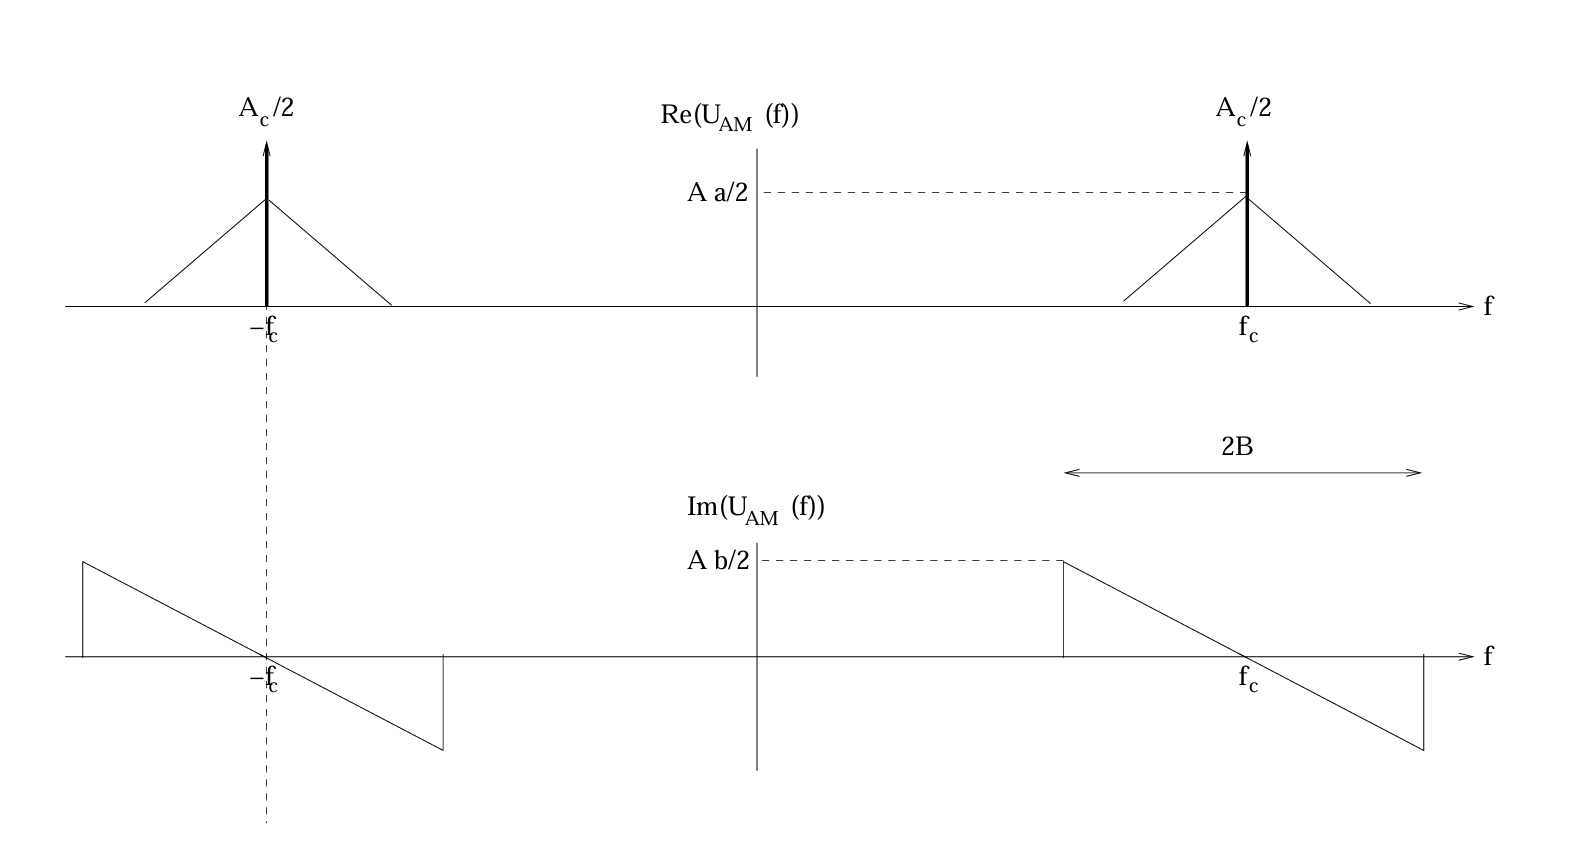
\includegraphics[width=1\linewidth]{Conventional_AM_spectrum.png}
    \caption{Spectrum of Conventional AM}
    % \label{fig:enter-label}
\end{figure}

The key concept behind conventional AM is that, by making \( A_c \) large enough, the message can be demodulated using a simple envelope detector. Large \( A_c \) corresponds to expending transmitter power on sending an unmodulated carrier which carries no message information, in order to simplify the receiver. This tradeoff makes sense in a broadcast context, where one powerful transmitter may be sending information to a large number of low-cost receivers, and is the design approach that has been adopted for broadcast AM radio. 

The key issue with conventional AM is its inefficiency in terms of power utilization. This led to the development of DSB-SC modulation which addresses these issues by suppressing the carrier and improving the power efficiency. 

  \[  u_{DSB}(t) = A m(t) \cos(2\pi f_c t) \]


Taking Fourier transforms, we have

   \[ U_{DSB}(f) = \frac{A}{2} \left( M(f - f_c) + M(f + f_c) \right) \]

   \begin{figure}
       \centering
       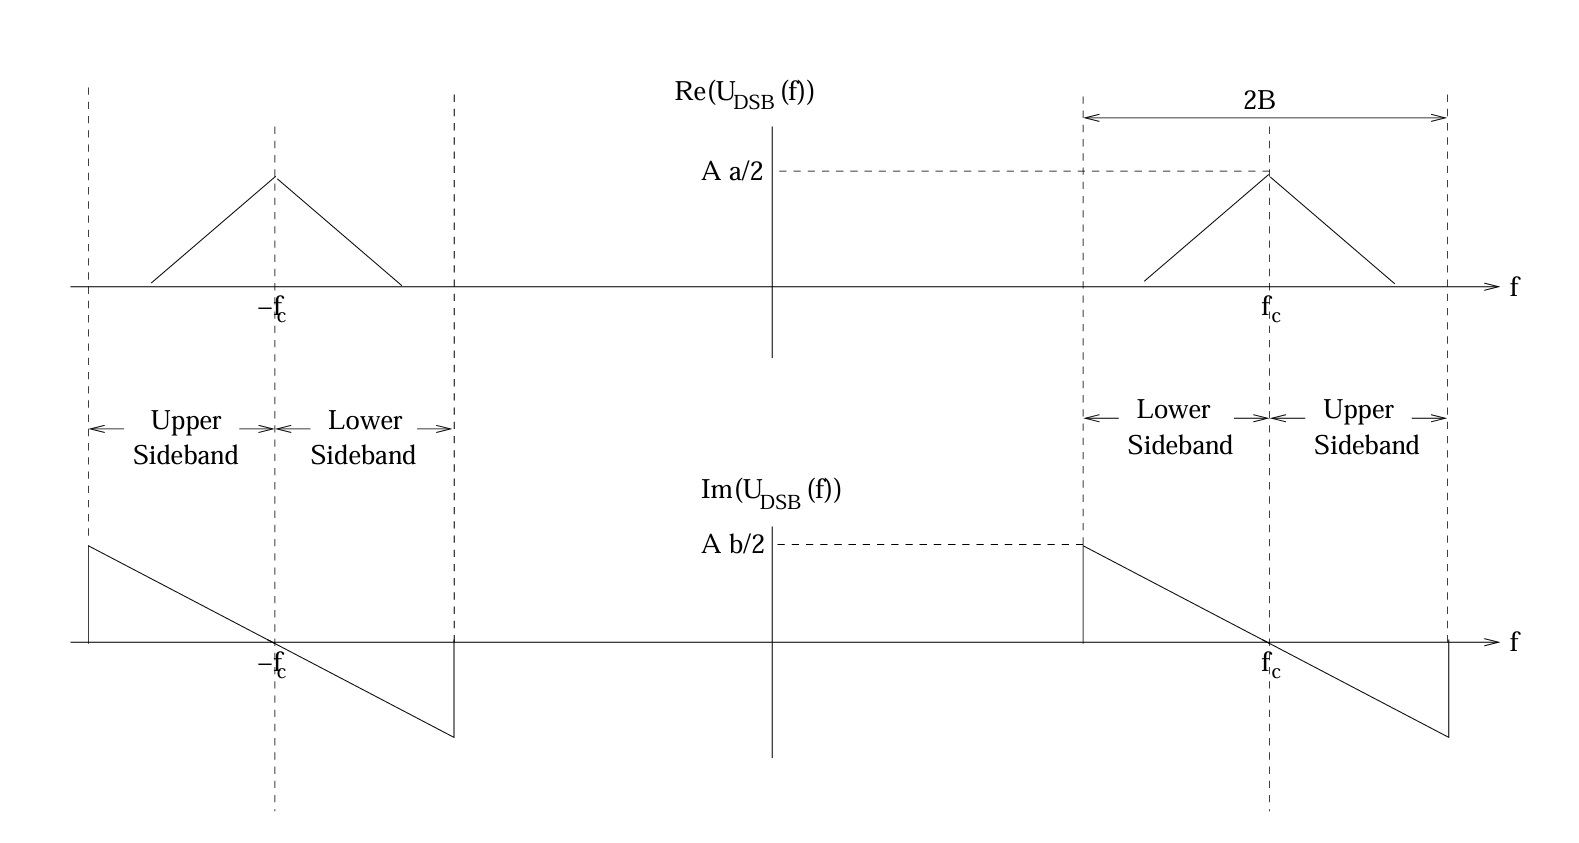
\includegraphics[width=1\linewidth]{DSB_SC_Passband_Spectrum.png}
       \caption{Caption}
       % \label{fig:enter-label}
   \end{figure}

\textbf{\textit{Demodulation: }}
\begin{figure}
    \centering
    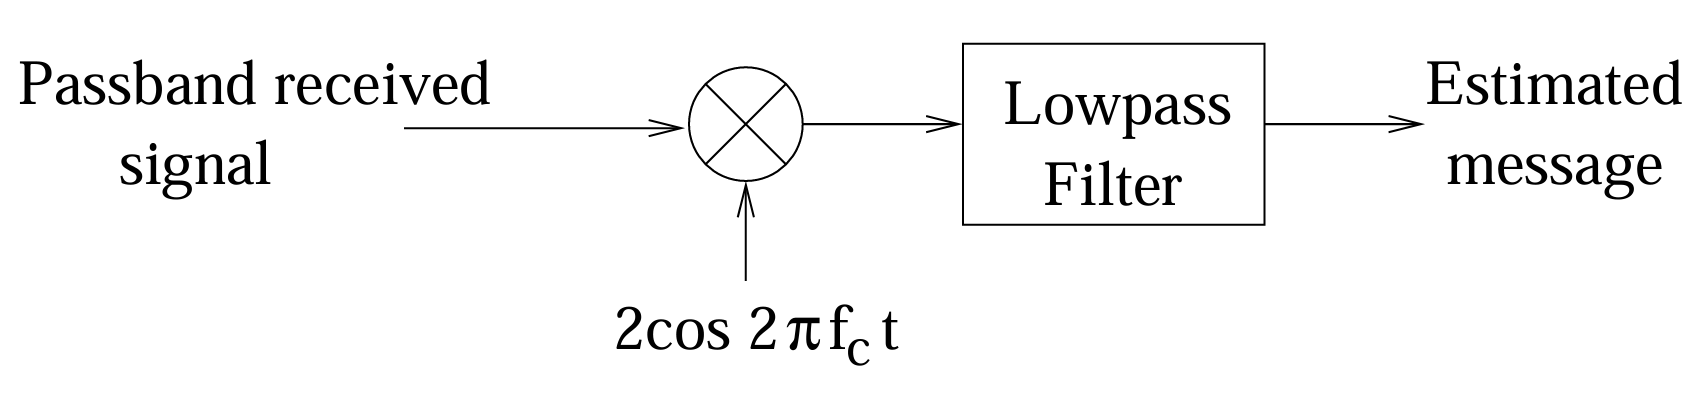
\includegraphics[width=1\linewidth]{Coherent_demodulation_AM.png}
    \caption{Caption}
    % \label{fig:enter-label}
\end{figure}

Multiply the received signal with the cosine of the carrier, and pass it through a low-pass filter. Ignoring noise, the received signal is given by
\[
    y_p(t) = A m(t) \cos(2\pi f_c t + \theta_r)
\]

where \(\theta_r\) is the phase of the received carrier relative to the local copy of the carrier produced by the receiver’s local oscillator (LO), and \(A\) is the received amplitude, taking into account the propagation channel from the transmitter to the receiver. In order for this demodulator to work well, we must have \(\theta_r\) as close to zero as possible; that is, the carrier produced by the LO must be coherent with the received carrier.

The effect of phase mismatch:
\[
    2y_p(t) \cos(2\pi f_c t) = A m(t) \cos(2\pi f_c t + \theta_r) \cos(2\pi f_c t)
\]

\[
=A m(t) \cos\theta_r + A m(t) \cos(4\pi f_c t + \theta_r)
\]

We recognize the second term on the right-hand side as being a passband signal at \(2f_c\) (since it is a baseband message multiplied by a carrier whose frequency exceeds the message bandwidth). It is therefore rejected by the low-pass filter. The first term is a baseband signal proportional to the message, which appears unchanged at the output of the LPF (except possibly for scaling), as long as the LPF response has been designed to be flat over the message bandwidth. The output of the demodulator is therefore given by
\[
    \hat{m}(t) = A m(t) \cos\theta_r 
\]

The demodulator output is proportional to the message, which is what we want, but the proportionality constant varies with the phase of the received carrier relative to the LO. In particular, the signal gets significantly attenuated as the phase mismatch increases, and gets completely wiped out for \(\theta_r = \frac{\pi}{2}\).

Note that, if the carrier frequency of the LO is not synchronized with that of the received carrier (say with frequency offset \(\Delta f\)), then \(\theta_r(t) = 2\pi \Delta f t + \phi\) is a time-varying phase that takes all values in \([0, 2\pi)\), which leads to time-varying signal degradation in amplitude, as well as unwanted sign changes. Thus, for coherent demodulation to be successful, we must drive \(\Delta f\) to zero, and make \(\phi\) as small as possible; that is, we must synchronize to the received carrier.




\section{Circuit Design \& Implementation}
\subsection{Local Oscillator}
Ref. from last year AEC project
\subsection{Modulator}
Ref. from last year mixer
\subsection{Demodulator}
mixer + LPF



\section{Experimental Setup \& Methodology}

\section{Results \& Performance Metrics}


\begin{enumerate}
    \item \textit{Detectability: }, i.e., the quality of the demodulated signal for a given amount of channel attenuation and receiver noise.
    \item \textit{Bandwidth efficiency: }, i.e., the bandwidth occupied by the modulated carrier for a given information rate in the baseband signal. This aspect plays a critical role in today's systems because the available spectrum is limited.  
\end{enumerate}


\begin{figure}
    \centering
    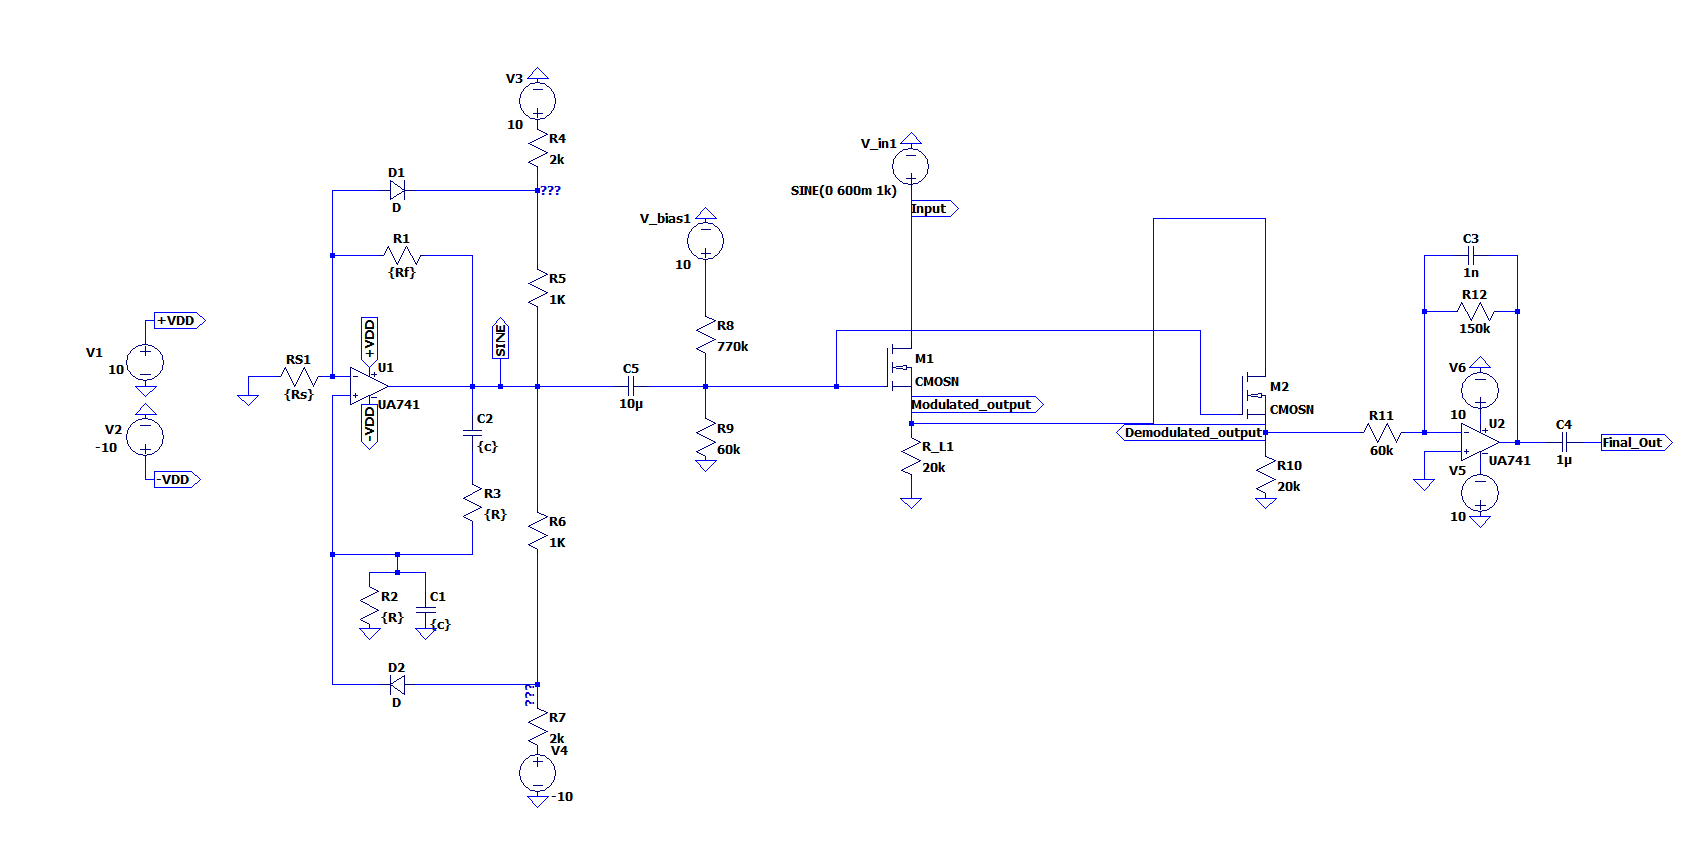
\includegraphics[width=1\linewidth]{Images/Full_circuit_ltspice.png}
    \caption{Caption}
    % \label{fig:enter-label}
\end{figure}

\begin{figure}
    \centering
    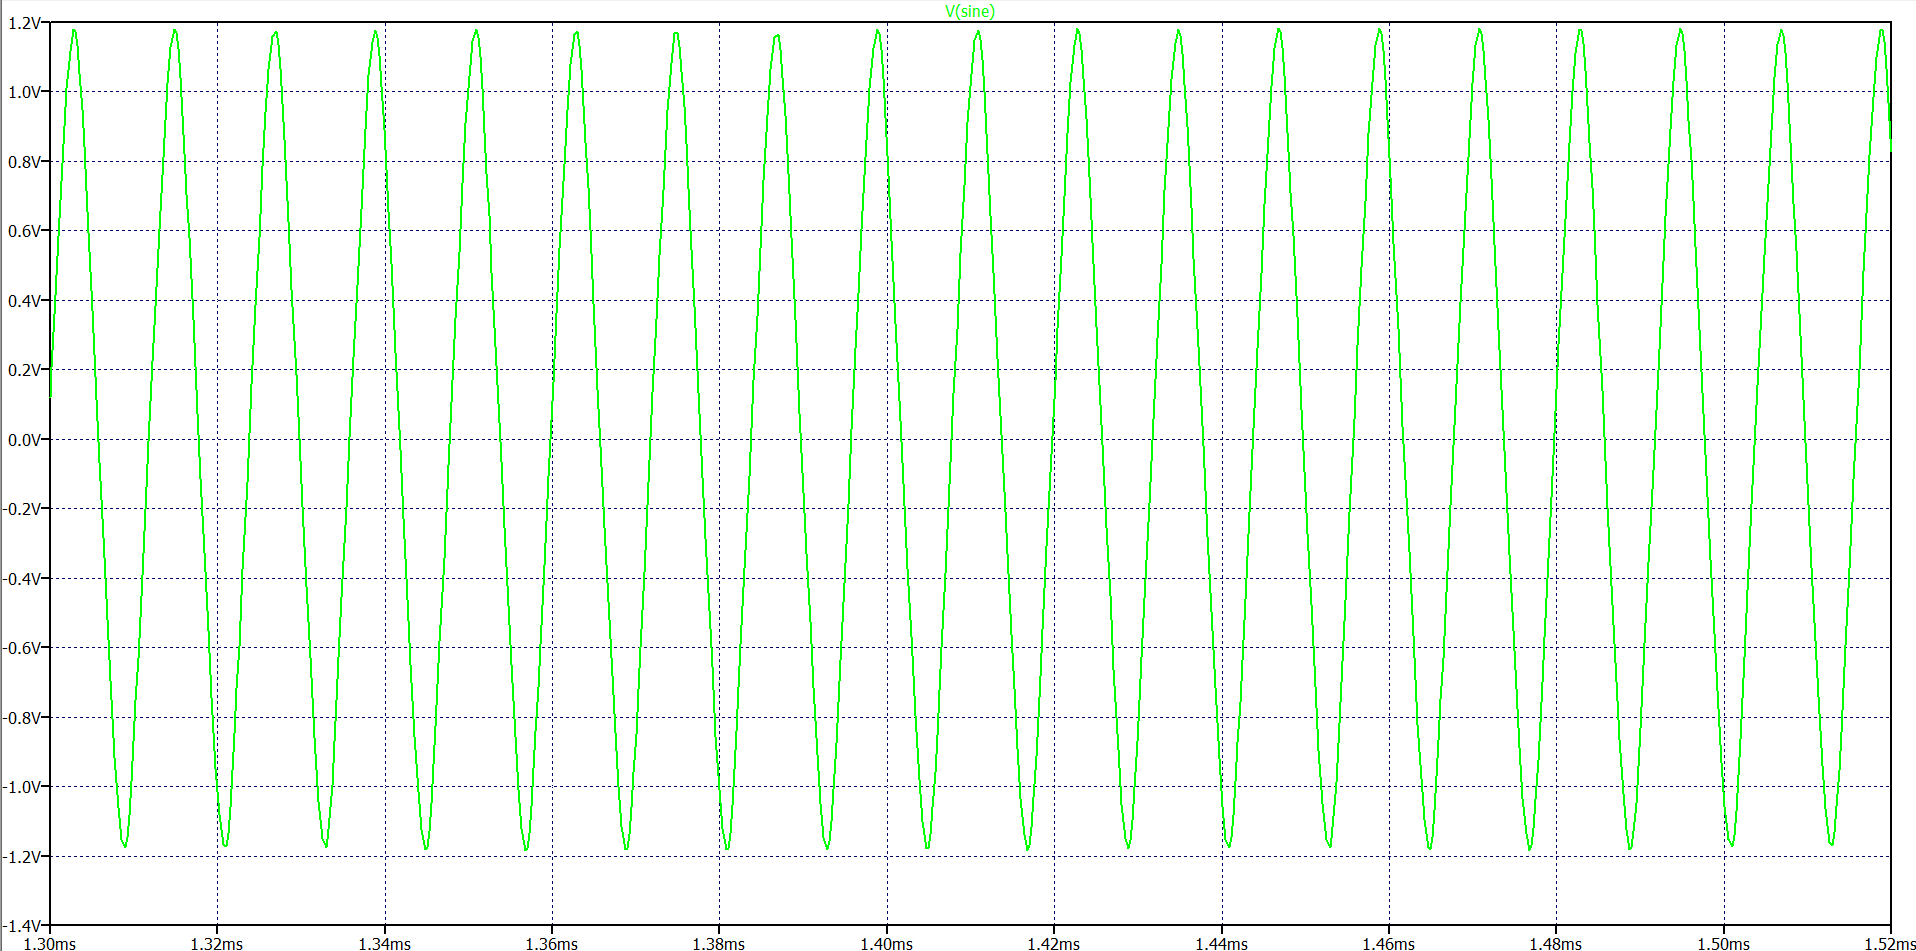
\includegraphics[width=1\linewidth]{Images/Osc_simulation.png}
    \caption{Caption}
    % \label{fig:enter-label}
\end{figure}

\begin{figure}
    \centering
    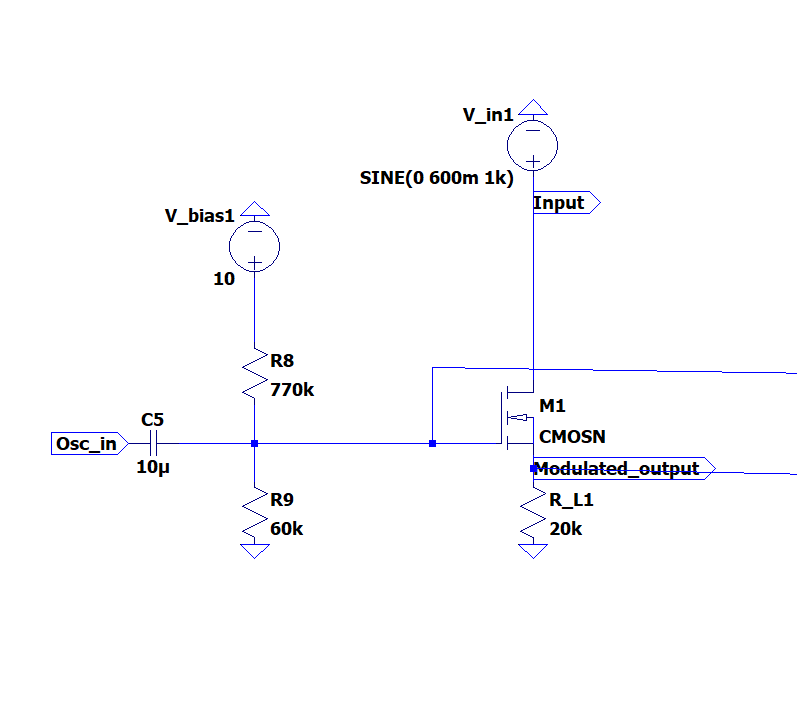
\includegraphics[width=1\linewidth]{Images/Modulator_ltspice.png}
    \caption{Caption}
    % \label{fig:enter-label}
\end{figure}

\begin{figure}
    \centering
    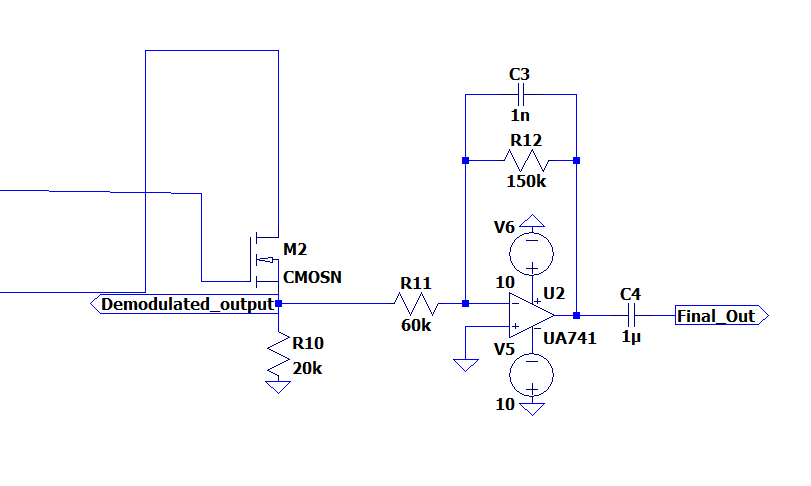
\includegraphics[width=1\linewidth]{Images/Demodulator_ltspice.png}
    \caption{Caption}
    % \label{fig:enter-label}
\end{figure}

\begin{figure}
    \centering
    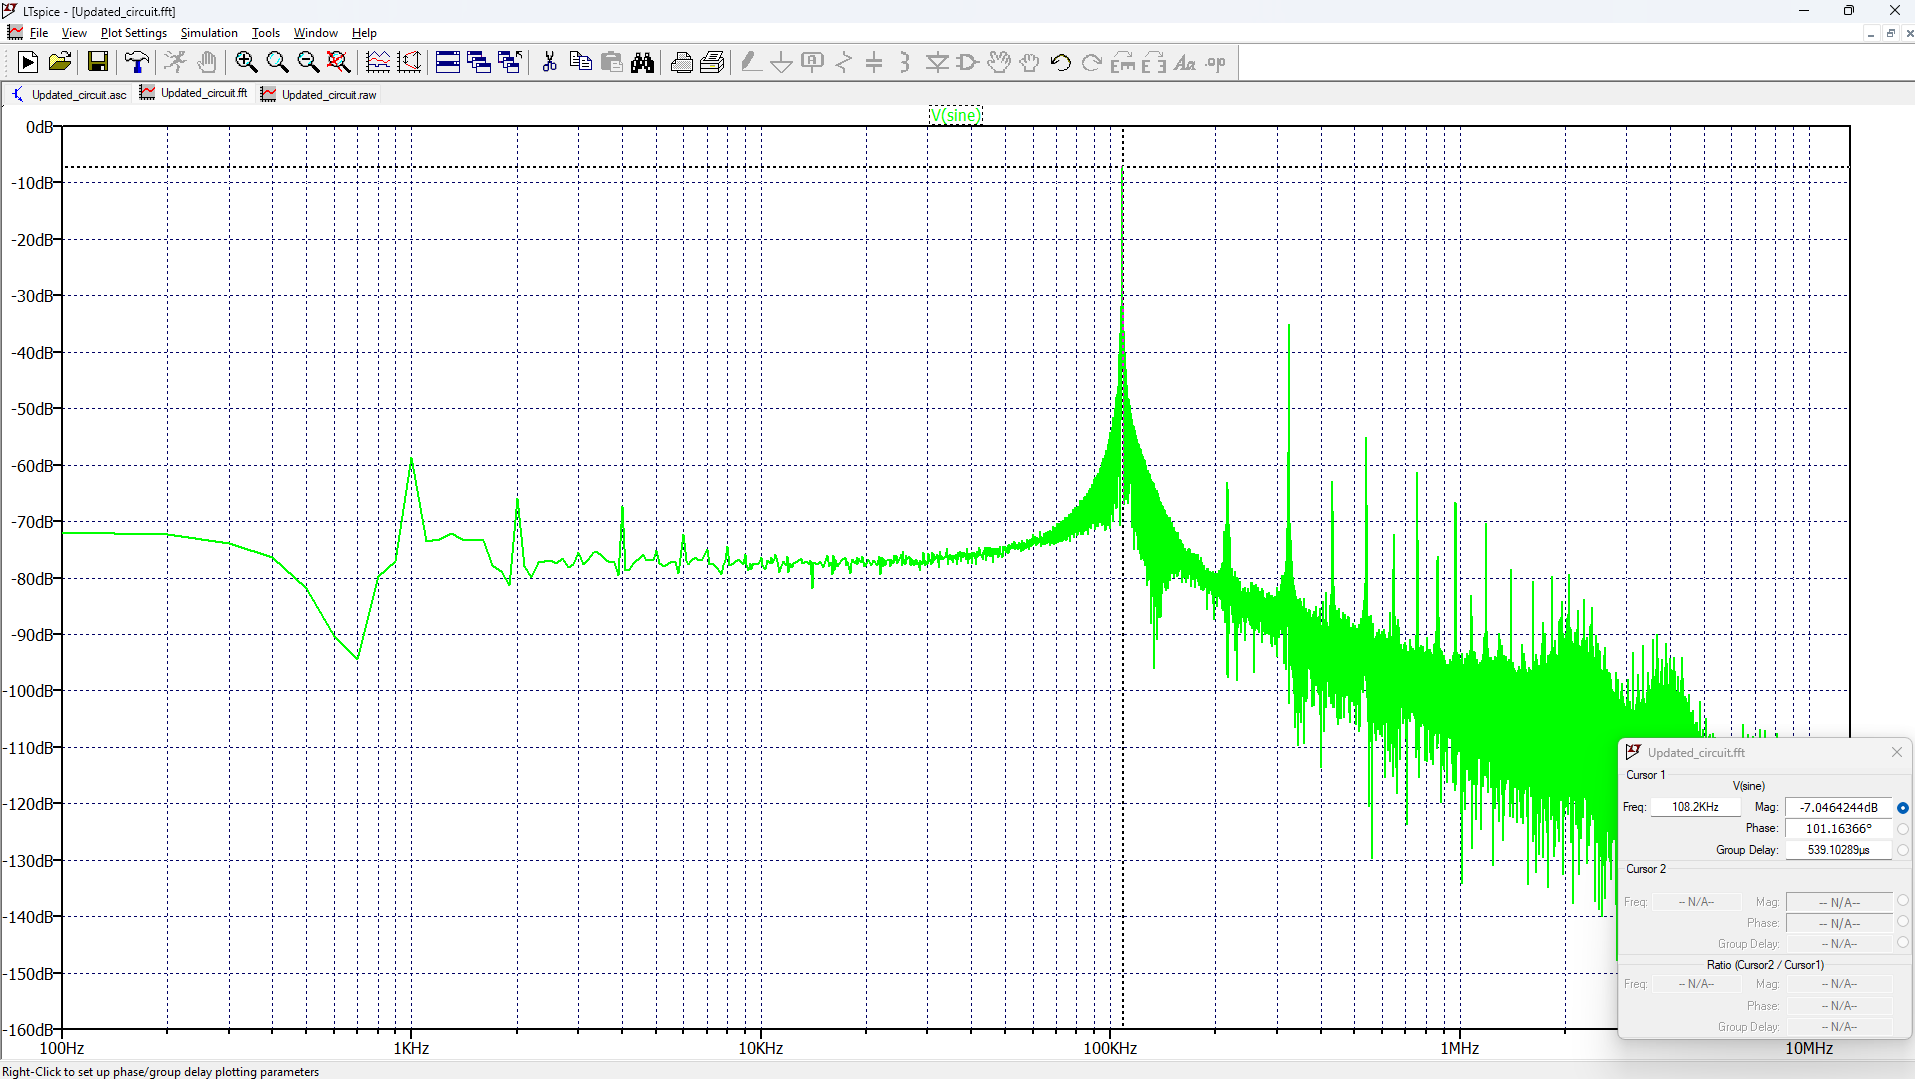
\includegraphics[width=1\linewidth]{Images/fft_sine_osc.png}
    \caption{Caption}
    % \label{fig:enter-label}
\end{figure}

\begin{figure}
    \centering
    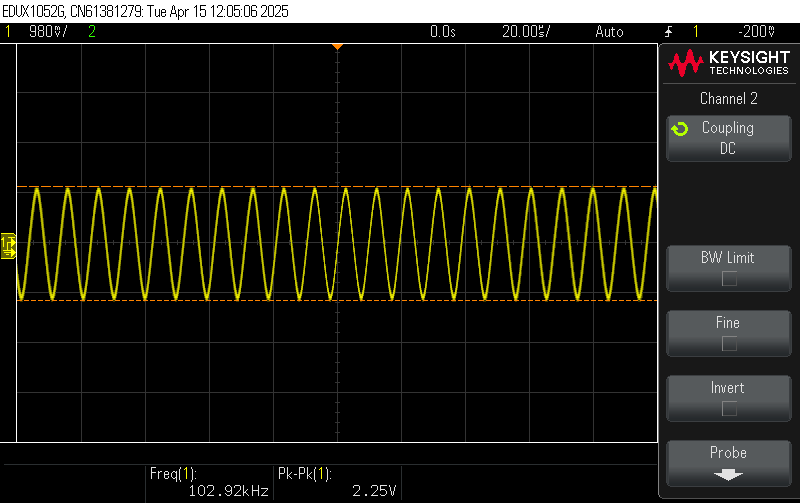
\includegraphics[width=1\linewidth]{Images/osc_circuit_out.png}
    \caption{Caption}
    % \label{fig:enter-label}
\end{figure}

\begin{figure}
    \centering
    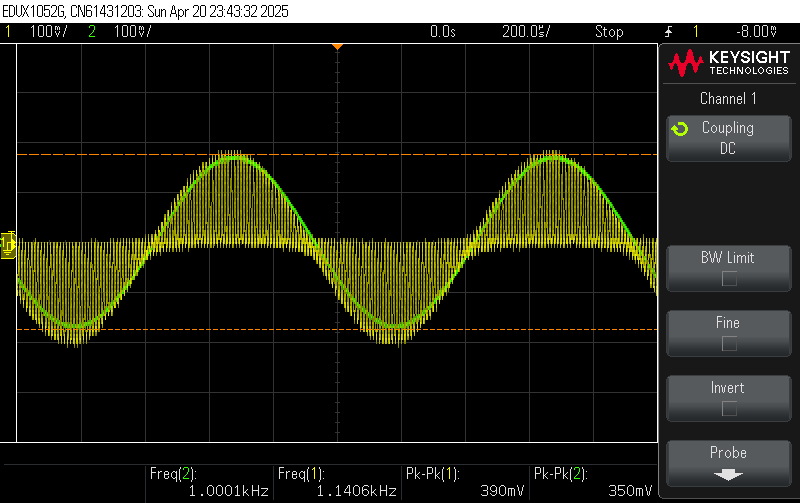
\includegraphics[width=1\linewidth]{Images/modulated_out_circuit.png}
    \caption{Caption}
    % \label{fig:enter-label}
\end{figure}

\begin{figure}
    \centering
    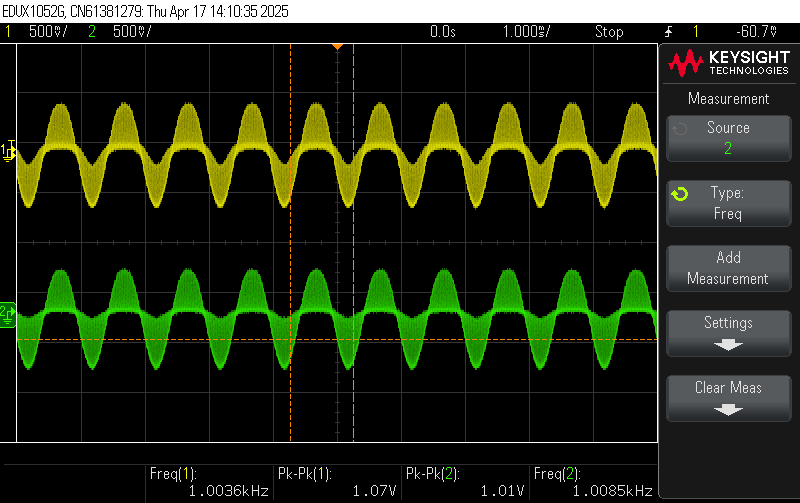
\includegraphics[width=1\linewidth]{Images/modulated_demodulated.png}
    \caption{Caption}
    % \label{fig:enter-label}
\end{figure}

\begin{figure}
    \centering
    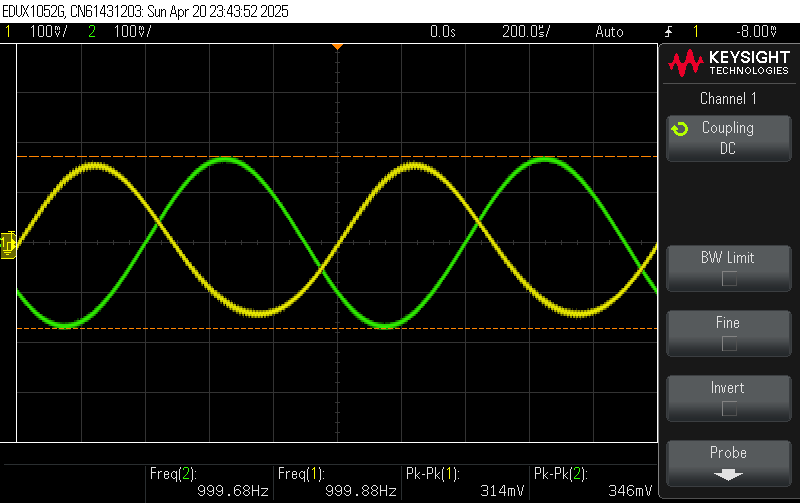
\includegraphics[width=1\linewidth]{Images/final_out_circuit.png}
    \caption{Caption}
    % \label{fig:enter-label}
\end{figure}

\begin{figure}
    \centering
    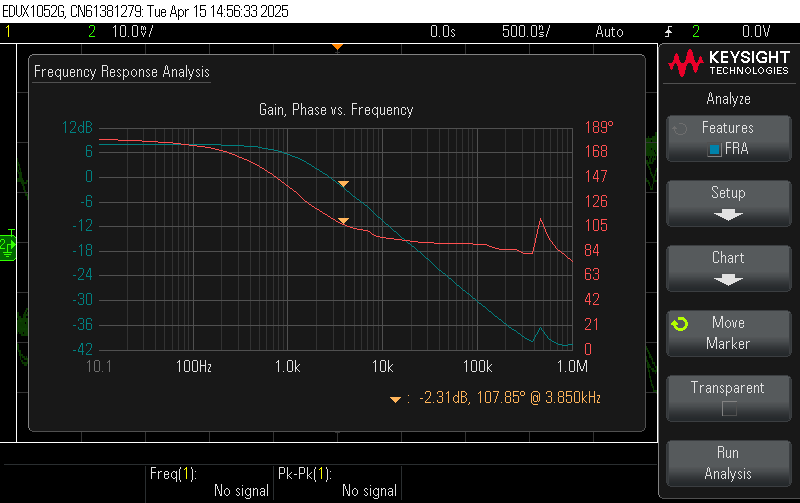
\includegraphics[width=1\linewidth]{Images/filter_response.png}
    \caption{Caption}
    % \label{fig:enter-label}
\end{figure}

\begin{figure}
    \centering
    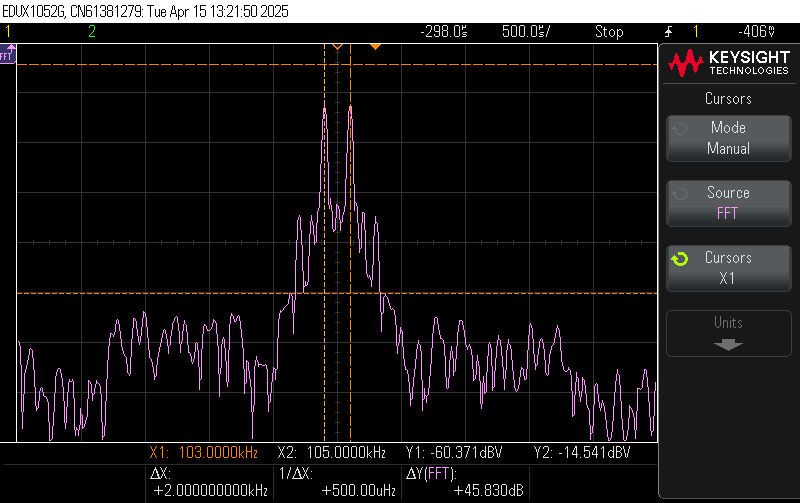
\includegraphics[width=1\linewidth]{Images/modulated_output_fft.png}
    \caption{Caption}
    \label{fig:enter-label}
\end{figure}
\section{Bonus Objectives}
\begin{itemize}
    \item Tunable LO using potentiometers
    \item Gilbert cell (for the mixer)
\end{itemize}

\begin{thebibliography}{00}
\bibitem{wiki-dsb}
\textit{Double-sideband suppressed-carrier transmission: }
\href{https://en.wikipedia.org/wiki/Double-sideband_suppressed-carrier_transmission}{Link}
\bibitem{wiki-AM}
\textit{Amplitude Modulation}
\href{https://en.wikipedia.org/wiki/Amplitude_modulation}{Link}
\bibitem{Text-book-Madhow}
\textit{"Introduction to Communication Systems" by Upamanyu Madhow}
\bibitem{Text-book-Razavi}
\textit{"RF Microelectronics" by Behazad Razavi}
\bibitem{RC-Phase-Shift}
\href{https://vesit.ves.ac.in/RC_phase_shift/theory}{\textit{Phase Shiftor Circuit}}
\bibitem{RC-Calculator}
\href{https://www.omnicalculator.com/physics/rc-circuit}{RC Resonant frequency calculator}
\end{thebibliography}
\end{document}
